\chapter{相关理论基础}
强化学习主要用于解决序贯决策问题,而
% 强化学习的目标是求解一个可以使得回报期望最大化的最优策略。
一般的序贯决策问题可以使用马尔科夫决策过程(Markov Decision Process, MDP)的框架来描述,在利用MDP将问题形式化后,又可以使用基于模型的动态规划方法和基于无模型的强化学习方法来解决该问题。特别地,在强化学习中,对于状态和行为空间较大的问题,往往采用值函数逼近的方法进行求解。本章会依次对它们进行简要的介绍。

\section{强化学习过程}
强化学习是机器学习的一个重要分支,它是从控制工程、心理学和运筹学等相关学科发展起来的,最早可以追溯到巴普洛夫的条件反射实验。但是,直到20世纪90年代初强化学习技术才得到重视,并随着强化学习理论的不断发展和完善,目前已经成为人工智能领域的研究热点,广泛应用于机器人控制、无人驾驶和游戏等方面。

强化学习主要用于解决序贯决策问题,所谓决策,是指面对特定的状态,采取什么样的行为,才能使的回报最大化;所谓序贯,是指需要连续不断的做出决策。所以,强化学习属于一种交互式的学习方法,主要是通过智能体(Agent)与环境不断交互,并从环境反馈的奖赏信息中进行学习,目标是最大化未来的累积奖赏。具体交互过程如图$\ref{fig:强化学习过程}$所示:
\begin{figure}[htbp]
\centering
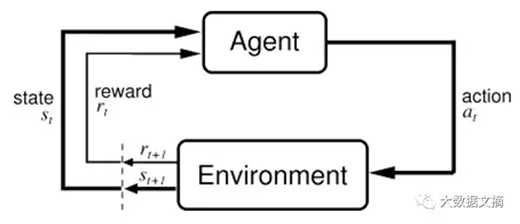
\includegraphics[width=0.6\textwidth]{强化学习过程}
\caption{强化学习的交互过程}
\label{fig:强化学习过程}
\end{figure}

(1)Agent感知当前的环境状态(state);

(2)根据当前的状态和奖赏值(reward),Agent会选择一个行为(action)并执行该行为;

(3)当Agent选择的行为作用于环境时,环境会转移到新的状态,并给出新的奖赏;

(4)Agent根据环境反馈的奖赏,计算回报值(return),并将回报值作为内部更新策略的依据。

 在这一过程中,Agent并不会被告知应该采取哪个行为,而只能经过不断的尝试后,根据得到的环境反馈信息做出判断。Agent选择行为的原则是:所选择的行为应该在以后的学习过程受到环境奖励的概率增大,受到惩罚的概率减小,也就是说,当前采取的行为和最终的目标有关。因为奖励信号是有延迟的,所以Agent有时候宁愿牺牲即时(短期)的奖励以获取更多的长期奖励。因此,试错搜索和延迟回报是强化学习中最重要的两个特征。

 从以上的描述中,可以看出,与监督学习不同,强化学习并不需要多样化的标签数据,而只需要带有回报的交互数据;另外,监督学习是一种反馈学习,即将模型的输出与标签之间所产生的误差信号反馈给模型来指导学习,而在强化学习中,由环境产生的奖赏信号是对所产生行为好坏的一种评价,Agent在行为与评价中获取知识,不断的改进行为方案以适应环境,并不是告诉Agent如何去产生正确的动作。


\section{强化学习的组成要素}
% 介绍马尔科夫决策过程,策略、累计回报、值函数、贝尔曼方程、最优值函数
\paragraph{马尔科夫决策过程}
强化学习可以使用马尔科夫决策过程框架来形式化的描述,MDP通常表示为一个四元组$<S,A,f,h>$,其中:$S$表示有限的状态空间,定义为一个有穷集合$\{ S_1,S_2,\cdots ,S_N \}$,$N$为状态空间的大小。$A$表示有限的行为空间,定义为一个有穷集合$\{ A_1,A_2,\cdots ,A_M \}$,$M$为行为空间的大小。$f$表示状态转移函数,$h$表示奖赏函数。

在马尔科夫决策过程中,考虑在任意的离散时间点$t$时,环境的状态为$S_{t}$,此刻Agent若采取行为$A_t$,就会得到有限的即时奖赏$R_{t}$,并且状态也会相应的转移到下一状态$S_{t+1}$。其中,奖赏$R_{t}$是根据奖赏函数$h$得到的,下一时刻的状态$S_{t+1}$是根据状态转移函数$f$得到的。另外,根据状态转移的情况,可以分为确定性状态转移和随机性状态转移。在确定性状态转移中,状态会转移到确定性的下一状态,而在随机性状态转移中,转移到的下一状态是不确定的,是一个随机变量。

% 又因为马尔科夫决策过程的状态具有马尔科夫性,因此状态转移函数和奖赏函数都仅和当前状态和行为有关,与历史的状态序列和行为序列无关。即:$p(s^{'},r|s,a) = Pr\{S_{t}=s^{'}, R_t=r|S_{t-1}=s, A_{t-1}=a\}$且$\sum_{s^{'}\in S}p(s^{'}|s,a)=1$,$\forall s\in S,\forall a\in A$。
\paragraph{策略和回报}
% \subparagraph{策略}
% 强化学习的目标是从给定的马尔科夫决策过程中,寻找最优的策略。
所谓策略是一个从状态到动作的映射,通常用符号$\pi$表示。
% 指在某一状态下,所采取的动作或所采取动作的概率,。
同样,策略也分为确定性策略和随机性策略,其中确定性策略定义为:$\pi$: $S \to A$ 输出的是一个动作序列,而随机性策略定义为:$\pi$: $S \times A \in [0,1]$ 输出的是该状态下所采取动作的概率:$\pi(s,a)=p[A_{t}=a|S_{t}=s]$。

% \subparagraph{回报}
强化学习的任务是从与环境的不断交互中,学习一个策略$\pi$,使其产生的累积奖赏(cumulative reward)最大化(即回报)。
% 当给定一个策略$\pi$时,如何进行策略的评估呢?此时便用到了累积奖赏的概念。
假设在时刻$t$后接收到的奖赏序列为$\{R_{t+1}, R_{t+2},\cdots\}$,那么采用折扣累积奖赏的方式计算回报可以表示为:
\begin{equation}\label{seq:reward}
G_{t}=\sum_{k=0}^{\infty}\gamma^{k}R_{t+k+1}
\end{equation}

式中,$G_{t}$为回报,$\gamma<1$,为一个常量,称为折扣因子。特别地,在系统与环境的交互过程中,如果任务可以自然地被分为带有终止时间片的片段,则该任务称为情节式(episodes)任务。如果任务无法分解成若干片段,整个任务需要不断的进行下去,则改任务称为连续式(continous)任务。

\paragraph{值函数}
当给定策略$\pi$时,在Agent的学习过程中,考虑评价某一状态的价值,很自然的想法是利用回报来衡量。但是,因为某一状态下的状态序列有很多,所以回报$G_{t}$是个随机变量,不是一个确定的值,无法作为目标函数进行优化。然而,其期望是个确定值,因此可以作为状态值函数的定义:当Agent采取策略$\pi$时,回报服从一个分布,将状态$s$的回报期望值定义为状态$s$的值函数。公式化为:
\begin{equation}
\label{seq2_vs}
v_{\pi}(s)=\mathbb{E}_{\pi}[G_{t}|S_t=s]=\mathbb{E}_{\pi}[\sum_{k=0}^{\infty}\gamma^{k}R_{t+k+1}|S_t=s]
\end{equation}

% Q函数是另一种评估值函数的方法。Watkins指出:。

在某些时候,记录状态行为对的值比只记录状态的值更有用。所以,状态行为值函数定义为在状态$s$下采取行为$a$的回报期望值,公式化为:
\begin{equation}
\label{seq2_qsa}
q_{\pi}(s,a)=\mathbb{E}_{\pi}[G_{t}|S_t=s,A_t=a]
=\mathbb{E}_{\pi}[\sum_{k=0}^{\infty}\gamma^{k}R_{t+k+1}|S_t=s,A_t=a]
\end{equation}

因为上述状态值函数\eqref{seq2_vs}的表达形式在实际应用中很不方便,因此,我们可以经过进一步的推导,得到状态值函数的贝尔曼方程:
\begin{equation}
\label{seq1}
\begin{aligned}
v_{\pi}(s)&=\mathbb{E}_{\pi}[G_{t}|S_t=s]\\
&=\mathbb{E}_{\pi}[R_{t+1}+\gamma G_{t+1}|S_t=s]\\
&=\sum_{a}\pi(a|s)\sum_{s^{'}}\sum_{r}p(s^{'},r|s,a)[r + \gamma\mathbb{E}_{\pi}[G_{t+1}|S_{t+1}=s^{'}]]\\
&=\sum_{a}\pi(a|s)\sum_{s^{'},r}p(s^{'},r|s,a)[r+\gamma v_{\pi}(s^{'})], \forall s \in S
\end{aligned}
\end{equation}
其中,$p(s^{'},r|s,a) = Pr\{S_{t+1}=s^{'}, R_{t+1}=r|S_{t}=s, A_{t}=a\}$,表示在状态$s$时执行行为$a$下,转移到下一个状态$s_{'}$并且得到奖赏$r$的概率。

同样地,也可以得到状态行为值函数的贝尔曼方程:
\begin{equation}
\label{seq2}
\begin{aligned}
q_{\pi}(s,a)=\sum_{s^{'},r}p(s^{'},r|s,a)[r+\gamma \sum_{a'}\pi(a'|s') q_{\pi}(s^{'},a^{'})], \forall s \in S, \forall a \in A
\end{aligned}
\end{equation}

计算值函数的目的是为了构建学习算法从数据中学习到最优策略,而每个策略对应着一个状态值函数,那么最优策略自然对应着最优状态值函数。所谓的最优状态值函数$v_{*}(s)$是指所有策略中值最大的值函数,即$v_{*}(s)==\max_{\pi}v_{\pi}(s)$,同样地,最优状态行为值函数$q_{*}(s,a)$为在所有策略中值最大的状态行为值函数,即$q_{*}(s,a)=\max_{\pi}q_{\pi}(s,a)$

因此,我们又可以由式\eqref{seq1}和式\eqref{seq2}进行推导(因为篇幅限制,推导过程略),分别得到最优状态值函数和最优状态行为值函数的贝尔曼最优方程:
\begin{equation}
\begin{aligned}
v_{*}(s)=\max_{a}\sum_{s^{'},r}p(s^{'},r|s,a)[r+\gamma v_{\pi}(s^{'})]
\end{aligned}
\end{equation}
\begin{equation}
\begin{aligned}
q_{*}(s,a)=\sum_{s^{'},r}p(s^{'},r|s,a)[r+\gamma \max_{a'} q_{\pi}(s^{'},a^{'})]
\end{aligned}
\end{equation}

最后,若求出了最优状态行为值函数,最优策略可以通过直接最大化 $q_{*}(s,a)$来决定:
\begin{equation}
\begin{aligned}
\pi_{*}(a|s) = 
    \begin{cases}
        1 & if \ a=\argmax_{a\in A}{q^{*}(s,a)},\\
        0 & otherwise.
    \end{cases}
\end{aligned}
\end{equation}

最后,需要强调的是:从公式\eqref{seq2_vs}和公式\eqref{seq2_qsa}可以看出,值函数是对未来奖赏的一种预测,对于一个状态$s$,如果它的奖赏很低,但并不意味着它的状态值就低,因为如果状态$s$的后续状态产生较高的奖赏,仍然可能得到比较高的状态值,这就是本文将强化学习技术用于求解营销问题,进而获取长期收益最大化的主要原因。但是,确定值函数需要Agent在其整个生命周期内通过一系列的观察,不断的估计才能得到。所以,我们接下来要做的就是如何快速而准确的获取值函数。

\section{强化学习经典算法}
根据是否依赖于环境,强化学习的求解方法可以分为基于模型的动态规划法和模型无关的强化学习算法。在基于模型的动态规划法中,需要提供精确的环境模型,然后根据环境的动态性利用贝尔曼方程迭代的求解值函数,其本质是动态规划(Dynamic Programming, DP)的思想,通过不断迭代直至稳定,得到精确解。模型无关的强化学习算法无需提供环境模型,根据agent与环境的不断交互收集样本,然后直接利用样本求解状态值函数和状态行为值函数。主要包括蒙特卡罗(Monte Carlo, MC)法和时间差分(Temporal Difference, TD)等算法。

\subsection{动态规划法}
动态规划法是指在给定模型的情况下,求解最优策略的方法。主要包括策略迭代和值迭代两种方法。

策略迭代算法包括策略评估和策略改善两个步骤,且两个步骤交替进行。在策略评估中,算法的每次迭代是建立在上一轮策略改善的基础上,对状态空间中的每个状态进行扫描,并利用贝尔曼方程进行更新,经过不断的迭代,值函数最终收敛至不动点。在策略改善中,算法利用上一轮策略评估得到的值函数,以贪心的方式生成一个新的策略。两
个过程不断交替,直至策略收敛至最终策略。特别地,贝尔曼方程$\eqref{seq1}$中状态值函数$v_{\pi}(s)$使用了其后继状态的值函数$v_{\pi}(s^{'})$来表示,这是自举(bootstrapping)的思想。

以行为状态值函数的策略迭代过程为例,:
\begin{displaymath}
\begin{aligned}
\pi_{0}\xrightarrow{E}q_{\pi_0}\xrightarrow{I}\pi_{1}\xrightarrow{E}q_{\pi_1}\xrightarrow{I}\pi_{2}\xrightarrow{E}q_{\pi_2}\xrightarrow{I}\pi_{3}\xrightarrow{E} \cdots \xrightarrow{I}\pi_{*}\xrightarrow{E}q_{\pi_{*}}
\end{aligned}
\end{displaymath}
其中$E$代表策略评估过程,$I$代表策略改善过程。初始时,策略和值函数都是随机的。在策略评估时,针对每一个状态行为值,使用贝尔曼方程$\eqref{seq2}$进行值函数的更新,直到$q_{k+1}$稳定便结束本轮迭代:
\begin{equation}
\begin{aligned}
q_{k+1}(s,a)=\sum_{s^{'},r}p(s^{'},r|s,a)[r+\gamma \sum_{a'}\pi(a^{'}|s^{'}) q_{k}(s^{'},a^{'})]
\end{aligned}
\end{equation}
在策略改善时,对所有的状态,使用贪婪方法求出新的策略:
\begin{equation}
\begin{aligned}
\pi_{k+1}(s)=\argmax_{a}q_{k+1}(s,a)
\end{aligned}
\end{equation}
在收敛到最优策略时,每一轮的策略都好于前一轮的策略。当策略$\pi$稳定时,迭代过程结束,即得到最优值函数$q_{*}(s,a)$和最优策略$\pi_{*}$。

值迭代算法是对策略迭代的简化,也包括策略评估和策略改善两个环节。与策略迭代不同的是,它不需要等到在策略评估值函数完全收敛时才进行下一次的迭代,而是对全部的状态行为空间每进行一次扫描(更新)就进行策略改善,加快了值函数的收敛速度。对每一个状态行为对,值迭代的更新公式如下:
\begin{equation}
\begin{aligned}
q_{k+1}(s,a)=\sum_{s^{'},r}p(s^{'},r|s,a)[r+\gamma \max_{a^{'}} q_{k}(s^{'},a^{'})]
\end{aligned}
\end{equation}
直到$q_{k+1}$稳定,算法结束。此时因为值函数已经收敛,直接对值函数使用贪心方法就可以得到最优策略。

\subsection{蒙特卡洛方法}
在求解强化学习问题时,由于动态规划法需要提供完整的环境模型且计算代价太大,限制了其在实际场景中的应用。当没有环境模型时,我们可以采用蒙特卡罗方法计算值函数,即用经验平均的思想代替随机变量的思想。其中,经验是指按照该策略做了很多次试验,产生很多情节(episode),每一个情节就是一次实验,平均就是指的平均值,按照求解方法不同又可以分为第一次访问(first-visit)蒙特卡罗方法和每次访问(every-visit)蒙特卡罗方法。在与环境的交互过程中,当一个情节结束后,则进行值函数的更新和策略的改善。另外,值函数的更新可采取可递增(Incremental )计算均值的方法,公式为:
\begin{equation}
\begin{aligned}
V_{k+1}(s)=V_{k}(s)+ \alpha(G_{t}-V_{k}(s))
\end{aligned}
\end{equation}
其中,$\alpha$为学习率,$G_{t}$为从状态$s$出发至情节结束所获的的累积折扣奖赏。

在动态规划中,为了保证值函数的收敛,算法会扫描状态空间的每一个状态。而蒙特卡罗方法想要充分评估值函数的前提是保证每个状态都可以被访问到,因此MC采用了探索性初始化(Exploring Start)的方法,即在每一个情节在迭代时,其初始状态都是随机分配的。

\subsection{时间差分方法}
相比于动态规划法,蒙特卡罗法使用了经验平均,虽然摆脱了对模型的依赖,但是不需要等到每个情节结束就可以进行值函数评估和策略更新,所以学习速度慢,学习效率不高。而动态规划因为使用了bootstrapping思想,所以可以在情节未结束时就可以根据未来值函数估计当前的值函数。时间差分法综合了两者的优点,融合了蒙特卡罗的采样方法和动态规划的bootstrapping思想。

所谓时间差分是指对同一事件或变量在连续两个时刻观测的偏差。TD(0)算法是指一步更新,即值函数直接根据下一个时间步进行学习,估计下一个状态的值函数。
假设在状态$S_{t}$时,Agent采取行为$A_{t}$,获得奖赏$R_{t}$的同时状态转移到$S_{t+1}$。因为环境从状态$S_{t}$向$S_{t+1}$以外的其它状态转移的概率为0,设$V(S_{t})$为最优$v_{*}(S_{t})$的估计值,那么状态$S_{t}$的值函数为:
\begin{equation}
\begin{aligned}
V(S_{t})=R_{t+1}+\gamma V(S_{t+1})
\end{aligned}
\end{equation}
时刻$t$的时间差分为:
\begin{equation}\label{shijiachafen}
\begin{aligned}
\delta_{t}=R_{t+1}+\gamma V(S_{t+1})-V(S_{t})
\end{aligned}
\end{equation}
那么,值函数的更新公式为:
\begin{equation}
\begin{aligned}
V(S_{t}) \gets V(S_{t})+\alpha (R_{t+1}+\gamma V(S_{t+1})-V(S_{t}))
\end{aligned}
\end{equation}
式中,$\alpha$为步长参数,控制学习率,$R_{t+1}+\gamma V(S_{t+1})$称为TD目标,$\delta_{t}=R_{t+1}+\gamma V(S_{t+1})-V(S_{t})$为TD偏差。

根据探索策略(行为策略)和评估策略是否为一个策略,可以将强化学习方法分为同策略(on-policy)和异策略(off-policy)两种方法。同样,时间差分方法也包括了同策略的Sarsa方法和异策略的Q-learning方法。在Sarsa方法中,行动策略和评估策略都是$\epsilon-greedy$的方法,对应的算法伪代码如$\ref{algo:algorithm_1}$所示。

\begin{algorithm}[htbp]
\small
\SetAlgoLined
\SetKwRepeat{Repeat}{Repeat}{until} 
% \KwData{this text}
% \KwResult{how to write algorithm with \LaTeX2e }
初始化$Q(s,a)$,$\forall s \in S$,$\forall a \in A$, 给定参数$\alpha$,$\gamma$\;
\Repeat{所有的$Q(s,a)$收敛}{
初始化起始状态$s$\;
根据$\epsilon-greedy$策略在状态$s$下选择行为$a$\;
\Repeat((对每个情节的每一步)){$s$是终止状态}{
	在状态$s$下选择行为$a$,得到奖赏$r$和下一个状态$s^{'}$\;
	在状态$s^{'}$下根据$\epsilon-greedy$策略得到动作$a^{'}$\;
	$Q(s,a) \gets Q(s,a)+\alpha[r+\gamma Q(s^{'},a^{'}) - Q(s,a)]$\;
	$s=s^{'}$,$a=a^{'}$\;
	}
}
输出最终策略:$\pi(s)=\argmax_{a}Q(s,a)$\;
\caption{Sarsa算法}
\label{algo:algorithm_1}
\end{algorithm}

与Sarsa方法不同,在Q-learning中,行为策略采用$\epsilon-greedy$策略,而目标策略采用贪婪策略,故又称为异策略Q-learning算法,其伪代码如$\ref{algo:algorithm_2}$所示。
\begin{algorithm}[htbp]
\small
\SetAlgoLined
\SetKwRepeat{Repeat}{repeat}{until} 
% \SetAlgoRefName{algorithm_2}
初始化$Q(s,a)$,$\forall s \in S$,$\forall a \in A$, 给定参数$\alpha$,$\gamma$\;
\Repeat{所有的$Q(s,a)$收敛}{
初始化起始状态$s$\;
% 根据$\epsilon-greedy$策略在状态$s$下选择行为$a$\;
\Repeat((对每个情节的每一步)){$s$是终止状态}{
	在Q函数中,根据$\epsilon-greedy$策略在状态$s$下选择行为$a$\;
	执行行为$a$后,得到回报$r$和下一状态$s^{'}$\;
	$Q(s,a) \gets Q(s,a)+\alpha[r+\gamma \max_{a} Q(s^{'},a)-Q(s,a)]$\;
	$s=s^{'}$\;
	}
}
输出最终策略:$\pi(s)=\argmax_{a}Q(s,a)$\;
\caption{Qlearning算法}
\label{algo:algorithm_2}
\end{algorithm}

在TD(0)中,更新当前值函数时,只用到了下一步状态值函数。而TD($\lambda$)考虑从未来的多步进行学习,并且采用加权的方法融合这多步的估计值,$\lambda \in [0,1]$决定了向未来观察的时间步长度。即
\begin{equation}
\begin{aligned}
V(S_{t} )\gets V(S_{t})+\alpha (G^{(\lambda)}_{t}-V(S_{t}))
\end{aligned}
\end{equation}
其中,
\begin{displaymath}
\begin{aligned}
G^{(\lambda)}_{t}=(1-\lambda) \sum_{n=1}^{\infty} \lambda^{n-1} G^{(n)}_{t}\\
\end{aligned}
\end{displaymath}
\begin{displaymath}
\begin{aligned}
G^{(n)}_{t}=R_{t+1}+\gamma R_{t+1}+ \cdots +\gamma^{n-1} R_{t+n}+\gamma^{n} V(S_{t+n})
\end{aligned}
\end{displaymath}

这就是TD($\lambda$)的前向视角表达形式,但是,这种方式需要等到整个实验结束才能计算。后向视角利用增量式的更新方式,不需要等到实验结束就可以更新当前状态的值函数,并且引入了资格迹$Z_{t}(s)$的概念,资格迹记录了最近被访问过的状态,也就是说,最近且最频繁被访问到的状态会被赋予最大的“资格”。更新方式为:

(1)首先,计算当前状态的TD偏差:$\delta_{t}=R_{t+1}+\gamma V(S_{t+1})-V(S_{t})$

(2)其次,更新资格迹:$Z_{t}(s) = 
    \begin{cases}
        \gamma \lambda Z_{t-1} & if s \neq s_{t},\\
        \gamma \lambda Z_{t-1}+1 & if s = s_{t}.
    \end{cases}$

(3)最后,对状态空间中的每个状态$s$,更新值函数:$V(s) \gets V(s)+\alpha \delta_{t} Z_{t}(s)$

综上,后向视角的时间差分方法不仅不需要环境模型,而且利用了增量在线的机制,实现方式简单有效,同时也保证了策略的实时性,被认为是强化学习中最核心的算法。

\section{值函数逼近方法}
至此,我们可以归纳出基于值函数的强化学习的基本步骤是:先评估值函数,然后再利用值函数改善当前的策略。其中,值函数的评估是关键。

在之前所介绍的强化学习方法中,值函数其实是一个表格,其索引是状态或者状态行为对,值迭代更新实际上就是这张表格的迭代更新,因此,这种强化学习称为表格型强化学习,它有一个前提条件:状态空间和行为空间都是离散的,并且状态空间和行为空间不能太大。然而,现实中的很多问题都具有很大的状态(行为)空间,甚至是连续的状态(行为)空间,比如围棋有 $10^{170}$  个状态空间,控制直升机飞行需要的是一个连续的状态空间。在这种情况下,需要我们利用函数逼近的方法表示值函数。从数学的角度来看,函数逼近方法可以分为参数化函数逼近和非参数化函数逼近,其中参数化函数逼近又分为线性参数逼近和非线性参数逼近。

\subsection{参数化函数逼近}
参数化函数逼近是从参数空间到值函数空间的映射,函数的形式和参数的个数事先由先验知识预设,而且参数是通过与目标函数有关样本数据来调整的。对于状态(状态行为)值函数可以由一组参数$\bm{\theta}\in \mathbb{R}^{n} $ 来近似,即:
\begin{equation}
\label{seq_2_3_2}
\begin{aligned}
&\hat{v}(s;\bm{\theta})\approx v_{\pi}(s)\\
&\hat{q}(s,a;\bm{\theta})\approx q_{\pi}(s,a)
\end{aligned}
\end{equation}

我们可以发现,在近似的状态值函数$\hat{v}(s;\bm{\theta})$中,针对每个状态,不再存储其状态值,而是只存储一组参数。把从已知的状态中到的值函数,推广至那些未碰及的状态中,这对于拥有大规模的状态空间来说,相当于对其状态空间进行了压缩。由于 $\bm{\theta}\in \mathbb{R}^{n}$,因此所需的存储开销为$O(n)$,当状态空间规模较大且均为离散时,$n$远远小于为每个状态存储值的开销$|S|$。

以状态值函数为例,我们可以得到目标函数为:
\begin{equation}
\label{seq:fun_approxi_obj}
\begin{aligned}
\argmin_{\bm{\theta}}(v_{\pi}(s)-\hat{v}(s;\bm{\theta}))^2
\end{aligned}
\end{equation}

即通过寻找参数向量$\bm{\theta}$,最小化近似函数$\hat{v}(s;\bm{\theta})$与真实函数$v_{\pi}(s)$的均方差。

值函数更新可以分为增量式学习方法和批学习方法。其中,随机梯度下降法是最常用的增量式学习方法。

由公式$\eqref{seq:fun_approxi_obj}$,我们可以得到参数的随机梯度更新公式为:
\begin{equation}
\begin{aligned}
\bm{\theta} \gets \bm{\theta}+\alpha[v_{\pi}(s)-\hat{v}(S_{t};\bm{\theta})]\triangledown_{\theta} \hat{v}(S_{t};\bm{\theta})
\end{aligned}
\end{equation}

进而,得到值函数的更新如下:
\begin{equation}
\label{seq:gradient}
\begin{aligned}
\triangle \bm{\theta} = \alpha (v_{\pi}(s)-\hat{v}(s;\bm{\theta})) \triangledown_{\theta} \hat{v}(s;\bm
{\theta})
\end{aligned}
\end{equation}

然而,公式$\eqref{seq:gradient}$并不能直接用于强化学习中,因为公式里有一个真实价值函数$v_{\pi}(s)$,或者是一个具体的数值,而强化学习没有监督数据。

从表格型值函数的更新过程中,我们可以看出无论是蒙特卡罗方法还是时间差分方法,都是朝着一个目标值更新的,这个目标值在蒙特卡罗方法中是$G_{t}$,在时间差分方法中是$R_{t+1}+\gamma Q(S_{t+1},A_{t+1})$,在$TD(\lambda)$中是$G^{\lambda}_{t}$。所以,如果将表格型值函数的更新过程推广至值函数逼近过程,那么,逼近值函数$\hat{v}(s;\bm{\theta})$的过程实际上可以看作是一个监督学习的过程,其数据和标签对为$<S_{t}, v_{\pi}(S_{t})>$,其中$v_{\pi}(S_{t})$等价于蒙特卡罗方法中的$G_{t}$,时间差分方法中的$R_{t+1}+\gamma Q(S_{t+1},A_{t+1})$,以及$TD(\lambda)$中是$G^{\lambda}_{t}$。因此,只要将公式$\eqref{seq:gradient}$总的$v_{\pi}(S_{t})$做相应替换就可以进行求解了。

在增量式学习方法学习方法中,每次更新模型需要与环境交互,数据使用一次即抛弃,导致样本使用效率不高。而所谓批方法是从给定一段时期的经验中抽取数据集:$D={<S_{1},v^{\pi}_{1}>,<S_{2},v^{\pi}_{2}>,\cdots,<S_{T},v^{\pi}_{T}>}$中,找到最好的拟合函数$\hat{v}(s;\bm{\theta})$,使的$LS(\bm{\theta})=\sum_{t=1}^{T}(v^{\pi}_{t}-\hat{v}^{\pi}_{t}(S_{t},\bm{\theta}))^2$ 最小,这种方法相当于经历重现(Experience Replay),把一段时期内的经历重新过一遍,更新参数,因此样本的利用效率高。

参数化函数逼近根据所使用逼近函数的不同,可分为参数化线性函数逼近和参数化非线性函数逼近两种。

以状态值函数为例,线性函数逼近可以表示为:
\begin{equation}
\begin{aligned}
\hat{v}(s;\bm{\theta})=\sum^{n}_{i=1}\phi_{i}(s) \bm{\theta}_{i}=\bm{\theta }^{T} \bm{\phi}(s)
\end{aligned}
\end{equation}
其中,$\bm{\theta}=(\bm{\theta}_{1},\cdots,\bm{\theta}_{n}) \in \mathbb{R}$,$\bm{\phi}(s)=(\phi_{1}(s),\cdots,\phi_{n}(s))^{T}$为状态$s$的特征向量,$\phi_{i}(s)$称为特征函数或者称为基函数,常见的基函数有:多项式基函数、傅立叶基函数以及径向基函数等。线性函数逼近不但形式简单、而且可以收敛到全局最优,缺点是表征能力较弱,而且基函数的形式需要事先选定,这也限制了函数的逼近能力。
% 但是正是由于其具备良好的收敛性和理论简单性,在强化学习的参数化方法中得到了充分应用。

在非线性函数逼近中,函数逼近器是关于参数$\bm{\theta}$的非线性函数。到在强化学习的应用场景中,一个状态数据是可能是持续流入的,而且下一个状态通常与前一个状态是高度相关的。因此,我们需要一个适用于非静态、非独立均匀分布的数据的训练方法来得到近似函数。在众多的非线性方法中,神经网络是最为符合的,因为它关于状态可导而且是迭代求解的。

神经网络可以看成是一种参数化基函数的方法。由于基函数的参数是从数据中学习得到的,因此其表示能力大大提升,神经网络的每层都可看成是基于上一层的新的基函数,也就是特征。从这个意义上说,后面一层是前面一层的抽象,这样可以对高维输入降维。

所以,和线性逼近器相比,非线性函数逼近的优点是有很强的表征能力和逼近能力,可以对目标函数以任意精度逼近,但是其收敛性难以保证,容易陷入局部最优,使的学术界对其的研究停滞了很长时间,直到2013年,DeepMind团队提出了一些改进的深度强化学习的训练方法,很大程度上解决了神经网络在强化学习问题中的收敛性问题,并且取得了令人振奋的实验表现,引发了针对此问题的新的研究热潮。具体细节可以参见本文第三章关于DQN的介绍。

\subsection{非参数化函数逼近}
在参数化函数逼近过程中,基函数的形式和参数的个数都需要提前设定,并且值函数的逼近效果很大程度上受到人为的经验的影响。而在非参数化函数逼近中,参数的个数以及基函数的形式并不是固定的,而是由样本决定,具有很高的灵活性。非参数化函数逼近方法包括基于核函数的方法和基于高斯过程的方法。因为本文第四章是使用的基于核函数的非参数化函数逼近的方法,所以此处仅对基于核的非参数函数逼近进行介绍。

基于核函数逼近模型可以表示为
\begin{equation}
\begin{aligned}
&\hat{q}(s,a;\bm{\theta})=\sum^{n}_{i=1}\bm{k}((s,a),(s_{i},a_{i}))\bm{\theta}_{i}\\
&\hat{v}(s;\bm{\theta})=\sum^{n}_{i=1}\bm{k}((s),(s_{i}))\bm{\theta}_{i}
\end{aligned}
\end{equation}
式中,$\bm{\theta}_{1},\cdots,\bm{\theta}_{n}$为参数向量,$\{(s_{i},a_{i})|i=1,\cdots,n\}$为样本集合,$\bm{k}:S\times A \times S \times A \to \mathbb{R} $为核函数。其中,常用的核函数有线性核函数、多项式核函数、径向基核函数以及Sigmoid核函数等。

利用核函数法逼近值函数的关键是能够将问题构造成一个带有核函数的优化问题。非参数化函数学习过程中完全依赖于样本,虽然带来一定的逼近灵活性,但是收敛性难以得到保证。

\section{本章小结}
 本章主要介绍了强化学习的相关理论基础知识。首先,对强化学习的整体交互过程进行简单介绍,让读者可以对强化学习有一个直观的认识和体会;接着,介绍了强化学习的框架马尔科夫决策过程以及强化学习的三个要素:策略、回报和值函数;然后,介绍了强化学习基于模型和模型无关的三种求解方法;最后,针对大规模问题,介绍了求解值函数的两种逼近方法:参数化函数逼近以及非参数化函数逼近。为后面章节做了铺垫。